%\documentclass[10pt,a4paper]{article}
%\usepackage[utf8]{inputenc}
%\usepackage{amsmath}
%\usepackage{amsfonts}
%\usepackage{amssymb}
%\usepackage{listings}
%\usepackage{graphicx}
%\author{Richard Torenvliet - 6138861}
%\title{Flood Simulation Browser}
%\maketitle

\section{Introduction}
This project concerns the Flood Simulation Browser. The concept of this browser is to illustrate/visualize a flood in a particular area. With this technology people can see the flow that the water will take. When a dike breaks it is important to know where the water will flow. Information about which locations in the area will be under water first can result in a successful evacuation plan. This system already exists, but is build for a multi-touch table only and is accessible by few people. This project aims on making it easier available and accessible. Which makes it more likely that someone with the right authority can take decisions about placing/reinforcing dikes or creating evacuation plans. Moreover, if this system is more accessible, then civilians of a certain neighbourhood that is threatened by water, have the ability to gain knowledge of where the water will go first. They then are able to take the the right crucial decisions based on this knowledge in the hour of need.

The implementation will be on a multi-touch device. In particular iPad and Android tablets. Users can use this application in an intuitive way and get more intelligence about the complex situation at hand. They have the ability to choose from several simulations that were already made for a specific area and also creating new simulations.
This document covers design choices/options in order to reach that goal. The first step is to get an idea of the existing simulation system of which this application will take use of. This includes a clarification of where this application is situated in the Urban Flood Project as a whole. The next step will be finding out the requirements of the tablet implementation, like which features does it have to contain in order to maintain intuitiveness. Just by showing the data would not be sufficient. The function of this App is to extend the simulation system with a use-ability and above all mobility factor.

A side assignment of this project is testing the scalability of the REST server. By testing how much requests the server can handle at ones it helps the urban flood project to estimate how many users can use the application at ones. The original multi touch application on the multi touch table was only one client. It's important to know that an early warning system stays online under the pressure more of clients.

The scientific research of this project will be the research for an intuitive design. The question will be, where do buttons, lists, and other important components need to be situated in an application. An other aspect of this project is the research for scalability of the server. This data will provide information about how many users can be handled by a server at once. The important part of this research will be the decision making of which framework or tool to use for the implementation of this application.

The first part of this document will describe the global information needed for the second part of this document. This division is made for  a simple reason. The ones that only care about the global information are served by the first part and the ones that are interested in how this application came to be are served in the second part of this document. Note that an understanding for how this application was made, the information of both parts are needed.

\part{Discovering the subject}
\section{Flood Simulation System}
The \emph{simulation} system already exists and runs in the cloud. That means it does all the calculation for the client and it's not important to know at which physical computer it runs. The system can calculate simulations by providing parameters about a certain area. For instance, the location and how much water you want to simulate. When a simulation is submitted and calculated, the simulation is stored. With http calls(GET or POST) to the system it returns a set of simulations that are present. The important thing to note is that the simulation consists of images that have to be displayed on a map, let's say Google Maps. The flood simulation system performs a complex simulation with the height map of the area. The height map holds detailed information about the height of an area. With this data, the flow of the water can be calculated and turned in to images. These images are used by the client application, this an important part of this project.
Not only does the system calculates the flow of water but it also calculates the estimated route that people take. It can calculate how much people would survive a simulated flood, keeping in mind that this project is all about saving people, this is interesting information.
 
\subsection{Flood API}
The API is a REST api that return JSON formatted string. The API functions as an interface to get the data of simulations and to start new simulations. It's a client server system where requests are done by the client and the appropriate data is transferred back to the client. With this data, information about a certain simulation can be displayed. The data can be in the form of an image or information in .csv files. The .csv files can be plotted and displayed in as a chart or graph. See part two for more information about the returned payloads.
New simulations are not done on the same server but done by HR Wallingsford 


\section{Flood Simulation App}
\subsection{Platform considerations}
As stated in the introduction the application is meant for tablets, but not specific for iOS or Android. How to maintain this demand on the application is one of the subjects of this project. This means that the application is not a native implementation and consists of one code-base and runs on more devices. There is a tool called PhoneGap \cite{PhoneGap} that uses HTML5, CSS3 and Javascript to build the app. In essence the developer builds a mobile website and PhoneGap can wrap this in an application. The native web-engine is used to render the mobile website. PhoneGap can result in a huge speed-up in development time, which is a huge advantage.  The speed up can be obtained by the fact that previously gained skills of webdevelopment can be re-used. Therefore there is no need to learn a new programming language or sdk for native apps. For example Objective C for iOS and Java for Android. The disadvantage can be that it feels like a mobile website in stead of a native application. In addition, the end product depends on the support of today's web-standards. Not all browsers have full support for HTML5 and CSS3, which forms the bases of a successful implementation of the application. For a list of supported elements, websites like caniuse.com \cite{CSS3} can be used to determine the percentage of support for a certain element/feature. But does not solve anything. Nevertheless, one disadvantage can be solved, a native feel of an application. For example, frameworks where native-like elements are created for you while coding in a programming language already known by a webdeveloper also exists.

This solution is Titanium Mobile, the Appcelerator \cite{Titanium-Appcelerator}. Titanium Mobile can build mobile applications that are in fact native applications. By programming in Javascript and call functions to create native elements the application can be created. The framework builds semi-native code, in the contrary to previously discussed PhoneGap. The development for this platform is fast and an application for both iOS and Android are quickly of the ground. But there is also a disadvantage by using Titanium. The applications are big, around 11MB no matter what. Because of the fact that the logic will still be in javascript(compiled), Titanium has to ship their javascript engine to the device. But not only do they take a lot of space on the storage device, it also has trouble with memory, see this blog-post\cite{memoryleak}. The blog-post discusses this issue, both developers and users discuss this issue in the reactions. Although this blog post refers to version 1.6 and 2.0 is already out, it's a threat to this project that can pop-up unexpectedly.

Moreover developing and testing on iOS provides expected behaviour and a large part of native elements are supported, for Android the native elements are mostly \textbf{not} the elements you thought they would looked like. To reach cross-platform apps the developer needs to constantly keep track if they're building an element for iOS or for Android. It might be stated that the functionalities of different platforms are not evenly supported. iOS is far out the most supported platform. Which only provides an advantage if the project only meant to run for iOS. The idea of Titanium Mobile is great, it works fine but will delay developing time when you truly want to reach crossplatform. Also, keeping in mind that this application needs a map that supports overlays(the simulation images). By searching trough the documentation \url{http://docs.appcelerator.com/titanium/2.1/index.html#!/api/Titanium.Map}, the only thing it supports is adding an annotation. An annotation is only a marker placed on the map with the ability to get de latitude and longitude of the marker. To sum this up, Titanium lacks support for both platform and map object, at the same time it can surprise the developer in an unpleasant  way by taking a lot storage and a buggy garbage collection.

Buillding crossplatform and creating native elements could mean a risk for completing the application. A browser is the only thing that ha s the most equality on both device, i.e. both Android's and iOS's native browser is based on the webkit browser. Webkit is an open source web engine that is used by both Safari and Chrome
\subsubsection*{Javascipt frameworks}
As already explained, PhoneGap only provides the possibility to create an app out of a website. This website can be build in any way the developer likes, using web technologies supported on the native device. There are frameworks that can speed up the development to make an intuitive application. Two frameworks that are considered are: jQuery Mobile \cite{jQuery-Mobile} and  Sencha Touch \cite{sencha}. 
\begin{description}
\item [jQuery Mobile]
This Javascript framework is build out of one Javascript file and one CSS file that the developer includes. By giving certain HTML elements a data attribute, which is a HTML5 element, the framework uses this to create views. A page is made by declaring a div adding data-role="page". Such a page can be given a footer like div data-role="footer". 
Switching frame one page to the other can be as simple as giving a html anchor a href to an id of a page. The figure \ref{fig:jquery} provides an example that will result in two pages, both pages have a button. Both buttons link to the other page (foo, bar), so tapping on one button will change the page to the other page.
\begin{figure}
\begin{lstlisting}
<div data-role="page" id='bar'>
	<a #href='foo' data-role="button">switch to foo</a>
</div>
<div data-role='page' id='foo'>
	<a #href='bar' data-role="button">switch to bar</a>
</div>
\end{lstlisting}
\caption{jQuery Mobile, pages example}
\label{fig:jquery}
\end{figure}

Creating two pages is quickly done, the downside of jQuery mobile is that in order to create an application where views look a like, you have to repeat yourself. You have to create pages with other id's and with the same look/elements but with different information. The conclusion is that jQuery mobile is that it is easy and the developer does indeed use HTML, CSS to create views.  But it is not easy to build a modular application. It is always possible to create such a modular application yourself, but when creating an application which is not such a framework the developer will run in to creating a framework in stead of the intended application.

\item [Sencha Touch 2]
Sencha touch 2 is a framework focused on the Model View Controller design pattern. It encourages the developer to use this pattern. The way of developing really differs from jQuery mobile. There where jQuery mobile sets you free to do whatever you like, sencha touch constraints the developer using components that are available in sencha touch. The difference can be easily explained with an example.

In the items array, see figure \ref{fig:sencha}, the items in that array can be anything supported by sencha touch like lists, a tabview, a map, etcetera. 

Sencha touch provides a command-line tool to build a starting environment. It creates files where the developer can start from. It's recommended to use this as a starting point. The advantage is an application that is structured out of the box with a design pattern that is the current standard(MVC). With Sencha Touch 2 there is no need for PhoneGap, unlike jQuery Mobile. Sencha Touch 2 provides the possibility to run the code on your simulator or native device with the command line tool. Testing for Android an iOS became much more simplistic resulting in less developing time. Running PhoneGap for Android, needs Eclipse to build, for iOS the developer needs to build in Xcode. When testing on both devices the developer needs to be able to test in both environments, and testing from the command-line is a lot easier than running both environments. 

A disadvantage of Sencha Touch could be, as seen in figure ~\ref{fig:sencha}, the syntax of sencha touch is not so easy at first. So the learning curve could be very steep.
The last argument that has a great influence on deciding which framework to use, could be that Sencha Touch provides an add-on that has the capability to create multi-touch charts. The original implementation of the urban flood browser on the multi-touch table has this feature. It would be a great extension of the project if this was possible. So with an eye on the future it could save a lot trouble, and it could add up to a more intuitive design. The next section will discuss this in more detail.
\pagebreak
\begin{figure}[h!]
\begin{lstlisting}
Ext.application({
    name: 'foo',

    launch: function() {
        Ext.create("Ext.tab.Panel", {
            fullscreen: true,
            items: [
                {
                    title: 'bar',
                    iconCls: 'bar',
                    html: 'bar'
                }
            ]
        });
    }
});
\end{lstlisting}
\caption{Sencha Touch application example. This example creates an application with the name 'foo'.  The html can be placed inside the items array. }
\label{fig:sencha}
\end{figure}
\end{description}

\vspace{1cm}
\subsection{Requirements Analysis}
\label{sec:requirements}
In short this involves the question, what does the application have to do? First of all, user needs to be able to see different simulations and be able to distinguish where certain simulations are located. Starting displaying the cities that are available as simulations would be the starting point of where the users can start interacting with the application. For displaying the cities a request to server is needed to  for displaying the cities. 
The cities are . The corresponding simulations have to be retrieved from the server and displayed in a list. Those list-items are the individual simulations, so it makes sense that when tapping on a list item, the simulation of the related item is going to be displayed. The form of these simulations are important. As previously stated, the simulations are in the form of images. These images are images from above and can be placed on the map. In order to display these images, there has to be a map available. Next, the latitude and longitude information is needed in order to place the image on the map.

As mentioned before, the floodsimulations are in the form of multiple imagery that are placed on the map. A requirement for these simulation images are that the user can control which image it wants to see in chronological sequence but of course does not decide the sequence is going to be. This requirement results in the need for controls for this feature. These controls need to be displayed somewhere in the viewport when the user has tapped on a list item of a simulation.

The flood simulations contain information about how much volume of water is present in a certain timestep. The simulations are divided in zones and labelled with an id. So a simulation contains information, this information needs to be displayed in such a way that it can be interpreted by the user. This would require a chart of some sort with the timesteps on the x-axis and some other value like volume on the y-axis. To determine the zone which contains the information, a latitude and longitude information is needed again. How this is done is described in part two of this document.


\subsection{App Design} 
\label{sec:appdesign}
The application will be used on tablets so a lot of space can be used. Working with tablets the screen gets larger than mobile phones. Which can result in a bigger travel distance of the user's hands. The GUI design has to be build with the considerations of the interaction capability of the users. For instance, unlike with mobile phones, according to Clark(2012) a leading designer in creating multi-touch applications, people intend to hold a tablet on the top halve of the tablet when holding with both hands, figure \ref{fig:perimeter}. The focus of the user is going from top to down. The top elements of the application will draw the first attention of the user. That's why Clark(2012) advises to place the important controls on the top half of the screen. The components that are important have to be placed in the left or right top of the screen. By taking Clark's advise the Flood Simulation Browser can be inspired.
\begin{figure}[h!]
\center
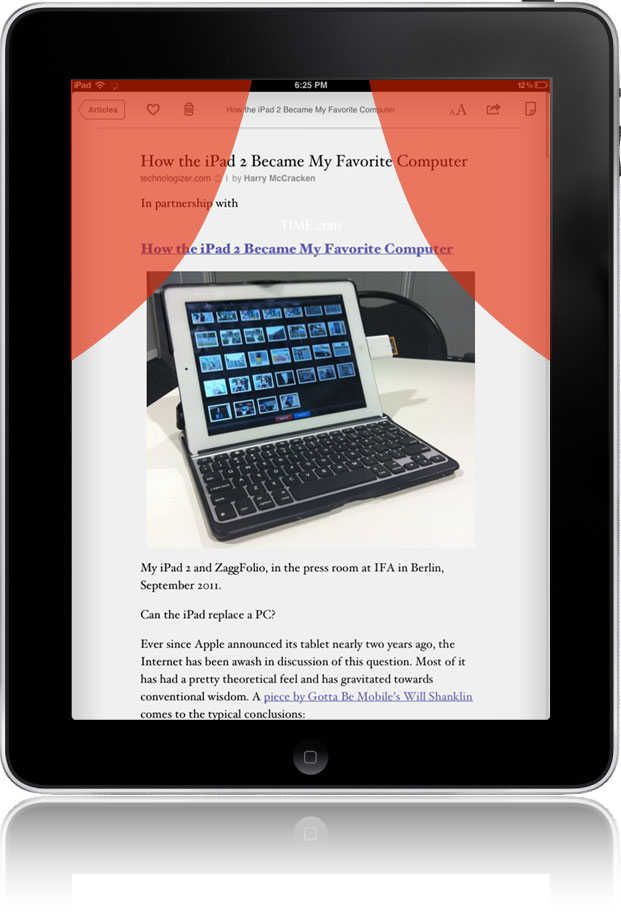
\includegraphics[scale=0.3]{touch.png}
\caption{Portrait touch perimeter(Clark, 2012)}
\label{fig:perimeter}
\end{figure}
First of all the flood simulations are within different cities. This can typically be a list of cities, also a list is scrollable and can be seen as an "infinite" array of cities around the world. Every city has it's own array of simulations to show. So it makes sense to also show these in a list. When a city is selected, the user has no use of the capability to select other cities and it's simulations. That's why the list of cities are pushed out of the viewport and the list of simulations is pushed in. 
It also makes sense to have one Map object in the view, where one city (latitude, longitude) can be shown at a time. The map object is the most important component of the browser. Inspired by Clark(2012) it can be stated that a hierarchy in importance of different view components can result in a different place on the screen. By placing the Map component always in the view and also as the biggest component, the idea of placing objects in a hierarchy of importance in the view is considered. For an example of this, see figure \ref{fig:mockup}.
The list component where cities and simulations are placed is the left side of the view, it could also be the right side but it would not matter. Since two hands are more or less symmetrical, so placing the list object left or right would not be a problem. It does matter concerning controls. Controls to change the timestep of a simulation are definitely needed. A simulation consists of multiple images on different time steps. By giving the user control of which image is seen at which time step is a crucial feature in the browser. Where and when(on which event) to place these controls is discussed in part two.
\begin{figure}[ht]
\center
\begin{tabular}{c}
	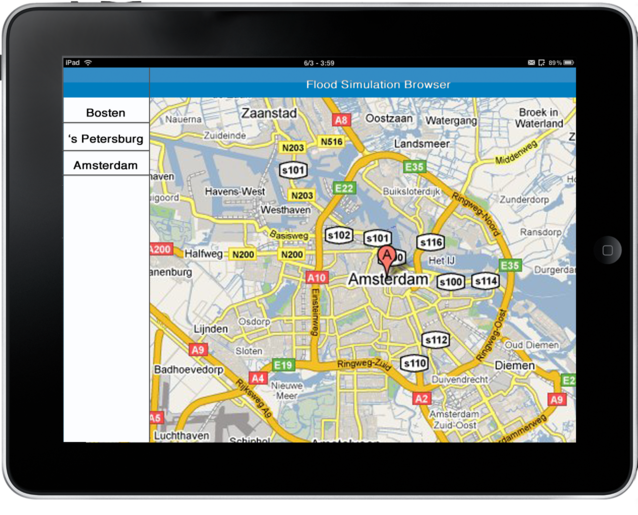
\includegraphics[scale=0.3]{mockup1_1.png} \\
	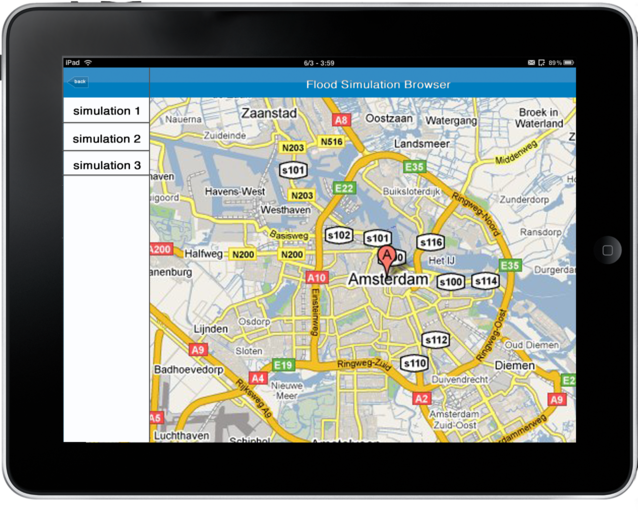
\includegraphics[scale=0.3]{mockup2_1.png}
\end{tabular}
\label{fig:mockup}
\caption{Cities list of which simulations are available}
\end{figure}

\begin{figure}[ht]
	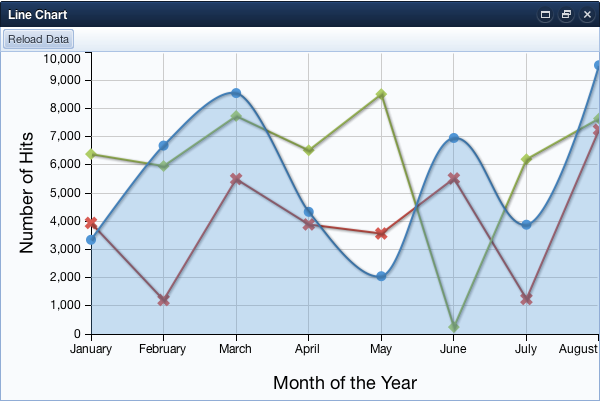
\includegraphics[scale=0.5]{chart.png} \\
\caption{Example of sencha chart}
\label{fig:sencha chart}
\end{figure}

The flood simulation browser that is already build for the multi-touch table has the ability to submit new simulations to be simulated in the cloud. The spot of the simulation can be arbitrary on the map, by simply touching a place on the map and alter some parameters, the cloud service can create a new simulation to be seen. Although this feature can be an seen as an extension of my project, with time left this feature can be build in. That's why it can be considered in the App's design. The controls of these parameters need to be somewhere in view, by placing this in the neighbourhood where the user touches the map could be intuitive. But not if it happens when the user is just navigating over the map, the user has to know that it is in the mode of with picking a place where to create a new simulation. The specification about these controls are discussed in the end report.

Furthermore, it's an important feature to display data of a simulation in certain area. The API provides this data. It holds information about how much water flows in that area over time. This data is the volume of water per timestep. The API requests latitude, longitude values, it then returns data of a location that is closest to this point. The application needs to display this data in a clear and understandable way. Charts are great way to display this data. In development of this application there needs to be a clear understanding of what usability is. Only displaying a chart of certain values could not be enough to learn anything or draw conclusions about the flood. The goal is to make use of the Sencha Touch Chart framework in order to provide comprehensive data of a flood in a certain area. See figure \label{fig:sencha chart} for an example of the chart framework.

\subsection{Scalability}
\label{sec:scalability}
A side assignment of the project is to test the scalability of the server. The server address is \url{sangkil.science.uva.nl}. To test this server it is needed to exclude any other parameter of the client. Such as maximum download speed, maximum throughput, latency of the network. The idea is not to test this at a home pc, but test it in a server that is hooked up in the same network as \url{sangkil.science.uva.nl}. More specifically, the connection between \url{mangkus.science.uva.nl}(hosted at the same location as sangkil) and \url{sangkil.science.uva.nl}. If this is the case the exclusion of restricted variables at client side could be possible. 
For stress testing the server a tool called siege \cite{Siege} would be of assistance. With this tool it is possible to launch requests to a url with $n$-nodes and $k$-connections executed per second. Siege registers the following data:
\begin{itemize}
\item Transactions - total hits
\item Availability - percentage of total succeeded hits
\item Elapsed Time - seconds
\item Data Transferred - MB
\item Response Time - seconds
\item Transaction Rate - seconds 
\item Throughput - MB/s
\item Concurrency - rate of concurrency
\item Succesful transaction - number of succeeded hits
\item Failed transactions - number of failed hits
\item Longest transaction - seconds
\item Shortest transaction - seconds
\end{itemize}
With this data new insight can be provided. By increasing the number of simultaneous connections, values could start to change. To really give the server a stress test, it's possible to provide a list of urls which can randomly be picked and executed. This simulates a more likely scenario and provides more insight on how the server would behave in a real situation. The expectation is that the response time might grow as the number of clients starts to grow. With more clients to serve, it could take longer if there are more clients active. If processor power is limited, maximum available memory is reached or even the implementation of the server for handling requests could all have an effect in the response time, or any other variable. The research for which variables changes, together with the cause and the solution is a part of this project and will be documented in the end report. 


%\section{Conclusion}
%The project will be implemented with the framework Sencha Touch 2. All encountered issues will be discussed in the end report. This %nformation can be used in future projects relating to creating cross-platform applications. Also all data about the scalability of the erver %will be documented. The urban flood project can in turn use this data in future plans to invest in more server power. If they do not need %to invest in more power this is also important.
%This project will ultimately result in a cross-platform application that can be used by the public or government to gain information %about a certain area.

\section*{End of Part one}
Part one describes the questions and some answers on what the approach of tackling this problem is going to be. For an understanding of what global problems are faced in this project, it will be sufficient to have read part one. Part two holds information about how the implementation is made, the problems that where discovered in process, results are displayed and discussed and ultimately ending with the conclusion of this project. 

\part{Describing the implementation}

\section{Server API}
A clear understanding of which request have to be done in order to gain the right information is needed first before beginning with any implementation. The full api is referenced in the appendix \ref{appendixA}. The appendix is referenced and used for explanations in the following sections.

\section{Sencha Touch 2}
The decision is fallen on Sencha Touch 2. Sencha Touch provides cross-platform capability and is based on web technology. Although Sencha Touch comes with a whole new syntax, based on Ext (reference!!), the content, look and logic is based on web languages.
Part one section \ref{sec:appdesign} the design of a touch application is discussed. The application is going to be created with the findings described in that section. Also the mockups \ref{fig:mockup} created early on in the project are great for keeping track on what the end goal should look like. 
%The requirements of the application discussed in section \ref{sec:requirements} are created in 

Sencha Touch is based on MVC with an addition of stores. Stores can hold information of whatever the application needs, more about this in a moment. The model is used for the communication with the database, the controller stands between the model and the view. The controller can steer between views and handle logic. The application has no direct need of models, since there is no database that has to be updated. Stores can handle enough communication between the server and the application. 

\subsection{Stores and Lists}
The stores in this application are prominently used for filling the lists. In particular the cities list en simulationslist. A list object is defined as the following. See appendix \ref{sec:area_api}.

\begin{figure}[h!]
\begin{lstlisting}
store = Ext.create('Ext.data.Store'{
    fields: ['name', 'corners', 'visbounds', 'area_id', 'center', 'size'],
	proxy: {
			type: 'rest',
			url: 'http://sangkil.science.uva.nl:8003/area/list.json',
			reader: {
				type: 'json',
				rootProperty: 'areas'
			},
		}
});
Ext.create('Ext.List', {
	title: 'locations',
	store: 'citystore',
	itemTpl: '<div>{name}</div>',
});
\end{lstlisting}
\caption{List of cities}
\label{fig:sencha}
\end{figure}
The store is automatically updated when the values change on the server. When something changes in the store, the list is also automatically updated. The specified fields are available in the list, containing the name of the field between brackets \texttt{\{ \}}, the field name of record $n$ is placed in list item $n$. Five stores are present in the application. \texttt{SimulationStore.js}, \texttt{SimulationDetailStore.js}, \texttt{LsmStore.js}, \texttt{SimulationsSummary.js}, \texttt{ChartStore.js}. 
\begin{itemize}
\item SimulationStore.js \\
Is sync with \url{http://sangkil.science.uva.nl:8003/area/list.json} on the server. Locally the store is in sync with the view List.js. Basically this store returns information of the simulation locations that are available. The most important data are the name, center, visbounds and area\_id. With the name for displaying in the list-item, the center for changing the map's center to the location of the simulation and visbounds are used for the image overlay. The area\_id is used in FloodDetailStore. When the user taps on a location, the data of longitude and latitude information is used to change the center of the map and push a new list over the current list. The second list holds information about which all the simulations available.
\item FloodDetailStore.js \\
Is in sync with multiple urls, \url{http://sangkil.science.uva.nl:8003/area/<area\_id>/info.json}, where the area is the area that is selected in List.js. This store adds information of dikes. The rest of the data is already present in the SimulationStore.js. The dikes consists of eight values, which are 4 corners with a latitude and longitude value. This means that a polygon can be formed from these four locations and displayed on the map.
\item LsmDetailStore.js \\
This store holds information of the population dynamics, meaning how the evacuation of the individuals will proceed. 
\item SimulationSummary.js \\
Syncs with \url{http://sangkil.science.uva.nl:8003/drfsm/list.json?summary}. This returns a json string that holds a list of all the simulations.Luckily a store can be filtered on a certain value. All the simulations have an area\_id specified. The store is filtered on the area\_id selected in List.js. Note that filters stay present, so before doing anything the store has to be cleared of all the filters.
\item ChartStore.js \\
This store is used for creating the chart. The chart expects a jsonStore with data and fields to plot. The data is retrieved from the server at run time of the application in \texttt{Api.js}.
\end{itemize}
\subsection{Layouts}

\subsection{Controller}

\subsection{Map}

\subsection{Creating Mockups in Sencha}

\section{Scalability}
The server \url{sangkil.science.uva.nl} is tested on scalability. An important part to notice when testing a server is how well it performs concerning how much peers it can serve and how the response time will change if the number of clients increases. By looking at the amount of clients that a server can serve is what scalability stands for. So how do the values change when connections, and therefore client numbers, start to rise.

To test the server, all bottlenecks at client side have to be brought done to an minimum. \url{mangkus.science.uva.nl} is the address of another server with the same specifications. The mangkus server is situated in the same server rack as sangkil. The TCP/IP package do not have to travel around the world in order to reach the destination, so the response time when not in a stress test could be in optimum state. 

\subsection{Testing}
So testing the sangkil server is done from the server mangkus. A tool siege is used for testing the server, previously discussed in section \ref{sec:scalability} in part one.
\begin{lstlisting}
$ siege -i -b -f file.txt -c $1 -r $2
\end{lstlisting}
 Testing is done by changing the concurrent processes and keeping the repetitions the same, or the other way around. That way a little grid search can be preformed to find a weakness in the server. The results of this search are discussed in the following sections.

\subsection{Results and Analysis}


\section{Conclusion}

\section{Discussion}

